\makeatletter
\def\input@path{{../../}}
\makeatother
\documentclass[../../main.tex]{subfiles}

\graphicspath{
	{../../img/}
	{../img/}
	{img/}
}

\begin{document}
\section{Комплекснозначные функции действительного переменного (КФ). 
Множество на комплексной плоскости}

\emph{Комплекснозначной функцией действительного переменного} (КФ) будем 
называть произвольное отображение
\begin{equation}
\label{lec25:1}
f: [\alpha,\beta ] \longrightarrow \C, \ \text{где}\;[\alpha,\beta ] \subset 
\R.
\end{equation}
В соответствии с \eqref{lec25:1} для 
$ \forall t \in  [\alpha,\beta ]\quad  \exists! f(t) \in \C$. Представим 
$f(t)$ в
параметрическом виде:
\begin{equation}
\label{lec25:2}
f(t) = x(t) + i y(t),\ \text{где}\  \begin{cases}
	x(t) = \Re f(t) \in \R, \\
	y(t) = \Im f(t) \in \R.
           \end{cases}
\end{equation}
\begin{exmp}
Пусть $z_0 = x_0 +  iy_0$, $x_0, y_0 \in \R$.

Рассмотрим некоторое $r \in \R, \ r > 0$. Тогда, учитывая, что $\forall z 
\in \C \implies d = |z-z_0|$ равно расстоянию между точками $z$ и $z_0$ на 
комплексной плоскости,
$ |z - z_0| = r$ соответствует множеству точек, равноудалённых
на расстояние $r$ от $\fix z_0$, т.~е. окружности с центром в $z_0$
 и радиусом $r$:
$|z -z_0| = \sqrt{(x-x_0)^2 + (y - y_0)^2} 
\implies (x-x_0)^2 + (y - y_0)^2 = r^2$.
Эту окружность можно параметризовать следующим
образом:
\[
\begin{cases}
	x = x_0 +  r\cos{t} \\
	 y=  y_0 + r\sin{t}
\end{cases} \quad t \in [-\pi, \pi].
\]
\[
\begin{cases}
	x = x_0 +  r\cos{t} \\
	 y=  y_0 + r\sin{t}
\end{cases} \implies z = x+ iy = x_0 + iy_0 + r(\cos{t} + i\sin{t}) = z_0 +
r{e}^{it}.
\]

Таким образом, получим следующую КФ:
\[
\begin{cases}
	f(t) = z_0 + r{e}^{it}, \\
	\quad t \in [-\pi, \pi].
\end{cases}
\]
\end{exmp}

Для КФ \eqref{lec25:1}, \eqref{lec25:2}  все основные свойства определяются
через соответствующие свойства $x(t)$ и $y(t)$ как действительных Ф1П.

Предел функции $f(t)$ определяется следующим образом: 
\[
\lim\limits_{t \to t_0}  f(t) = P = A + iB \in \C \iff
\begin{cases}
	\lim\limits_{t \to t_0}  x(t)  = \Re P = A \in \R \\
	\lim\limits_{t \to t_0}  y(t)  = \Im P = B \in \R
\end{cases} 
\]

Из этой равносильности следует, 
что  все основные свойства сходящихся Ф1П,
арифметические операции над сходящимися Ф1П автоматически переносятся на КФ.
В частности, функция \eqref{lec25:1} непрерывна в $t_0 \in [\alpha,\beta ]$,
если
\[\exists \lim\limits_{t \to t_0}  f(t) = f(t_0) \iff 
\begin{cases}
	\lim\limits_{t \to t_0}  x(t)  = x(t_0), \\
	\lim\limits_{t \to t_0}  y(t)  =  y(t_0).
\end{cases}\]

КФ будем считать дифференцируемой в $t_0 \in [\alpha,\beta ]$,  если 
$\begin{cases}
	\exists x'(t)  \in \R, \\
	\exists y'(t)  \in \R.
\end{cases}$ Производную КФ будем определять следующим образом:
\[
	f'(t) = x'(t) + iy'(t) \in \C.
\]

Если $f(t)$ дифференцируема для $\forall t_0 \in E \subset [\alpha,\beta ]$, 
то она считается дифференцируемой на $E$ (на концах 
подразумевается односторонняя дифференцируемость,
определемая как существование соответствующих 
односторонних производных для $x(t), \ y(t)$).

Если $\begin{cases}
	\exists \int\limits_{\alpha}^{\beta} x(t)\;dt  \in \R \\
	\exists \int\limits_{\alpha}^{\beta} y(t)\;dt  \in \R
\end{cases},$ то по определению полагаем
$\int\limits_{\alpha}^{\beta} f(t)\;dt = 
\int\limits_{\alpha}^{\beta} x(t)\;dt + i\int\limits_{\alpha}^{\beta} 
y(t)\;dt$.
Интегрируемые КФ (и интегралы КФ) обладают
основными свойствами, аналогичными 
свойствам интегрируемых Ф1П (и ОИ).
\begin{exmps}

\;

\begin{enumerate}
\item\[\begin{cases}
	f(t) = e^{iat} \\
	a = const \in \R
\end{cases}\!\! t \in [\alpha, \beta]
\qquad
\eqref{lec25:2} \iff 
\begin{cases}
	x(t) = \cos{at} \\
	y(t) = \sin{at}
\end{cases}  
\]
\[\begin{cases}
	\exists x'(t) = -a\sin{at}  \\
	\exists y'(t) = a\cos{at}
\end{cases}\implies \exists \left(e^{iat} \right)' = -a\sin{at} + ia\cos{at} =
 ia(\cos{at} + i\sin{at}) = iae^{iat}.
\]
\item\[
\int\limits_{\alpha}^{\beta}e^{iat}\;dt =
\int\limits_{\alpha}^{\beta}e^{iat}\cos{at}\;dt +
 i\int\limits_{\alpha}^{\beta}\sin{at}\;dt = 
 \frac{\sin{a\beta} - \sin{a\alpha}}{a} -   
 i\ \frac{\cos{a\beta} - \cos{a\alpha}}{a} = \]\[
= \left[ \frac{-i{e}^{iat}}{a} \right]_{\alpha}^{\beta}= 
\left[ \frac{{e}^{iat}}{ia} \right]_{\alpha}^{\beta}.
\]
\end{enumerate}
\end{exmps}

\begin{wrapfigure}{r}{0.4\textwidth}
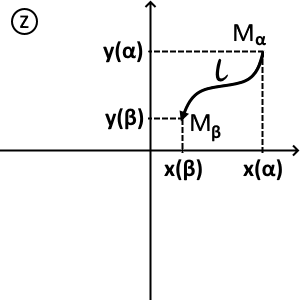
\includegraphics[width=0.4\textwidth]{lec25_1.png}
\end{wrapfigure}
На комплексной плоскости \textcircled{z}  КФ \eqref{lec25:2} соответствует
некоторая кривая $l$, ограниченная точками $
\begin{cases}
	M_{\alpha} = (x(\alpha), y(\alpha)), \\
	M_{\beta} = (x(\beta), y(\beta)).
\end{cases} $ Движение от $M_{\alpha}$ к $M_{\beta}$ будем называть 
\emph{положительным}. Таким образом мы получили положительно
определённую кривую $l^+$. Аналогично определяем отрицательно
определённую кривую $l^-$.

Если  $M_{\alpha} = M_{\beta}$, то кривая $l$ будет замкнута. 
Замкнутую кривую  $l$ будем называть \emph{замкнутым контуром},
если $l$ не имеет самопересечений и функция непрерывна. В общем
случае, замкнутую кривую  $l$ с движением против часовой стрелки
будем называть \emph{положительно ориентированной}, 
а по часовой~---
\emph{отрицательно ориентированной}. По аналогии  с $\R^2$,
 на комплексной плоскости  \textcircled{z} будем рассматривать следующие  
 простейшие множества:

Пусть $z_0\in \C - \fix,\ k \in \R,\ k > 0$.
\begin{enumerate}
\item Окружность: \[  |z - z_0| = k\] 
\item Замкнутая $k$-окрестность $z_0$ : \[ |z - z_0| \leq k\] 
\item Открытая $k$-окрестность $z_0$ : \[ |z - z_0| < k\] 
\end{enumerate}

Для множества $D$ на \textcircled{z} точку $z_0$, принадлежащую  $D$, 
будем называть \emph{внутренней для  $D$}, если существует открытая 
$R$-окрестность точки $z_0$ (будем обозначать ее
$B_R(z_0) = \{ z\ |\  |z - z_0| < R \}$), которая целиком входит в  $D$.
Если в каждой открытой окрестности точки 
$z_0 \in \C$ присутствуют как точки, принадлежащие $D$, 
так и точки, не принадлежащие ему, то точка $z_0$ называется 
\emph{граничной для $D$}.
Множество граничных точек $D$ будем обозначать $\sigma\!{D}$ и 
называть \emph{границей $D$}.
Граничные точки могут как входить, так и не входить в $D$. Для $z_0 \in \C$
последовательность
$(z_n),\ n\in\N$ называется \emph{последовательностью Гейне}, если $\forall
z_n\neq z_0, \ z_n \underset{n \longrightarrow \infty}{\longrightarrow} z_0 $.
 Точка $z_0 \in \C$ называется \emph{предельной для $D$},
если для нее существует последовательность Гейне $(z_n) \subset D$. Как и в
действительном случае, можно показать,
 что $z_0$ --- предельная для $D \iff
 \left[\begin{aligned} 
  z_0 \text{ --- внутренняя} \\
  z_0 \text{ --- граничная}
\end{aligned}\right. \ \text{для}\ D$. Иными словами, $z_0 \in \overline{D}$, 
где
$\overline{D} = \sigma\!{D}\cup D$ --- \emph{замыкание} множества $D$.
 Множество $D$ называется \emph{замкнутым}, если все граничные точки $D$
 входят в $D$ (иначе говоря, $D = \overline{D}$). 
Если в $D$ можно $\forall m, n \in D$ соединить некоторой непрерывной линией,
соответствующей некоторой
 КФ $z(t)$, целиком лежащей в $D$, то множество $D$ называется  \emph{связным}.
Связное множество $D$, не являющееся замкнутым, будем называть \emph{областью}.
Если связное множество замкнуто, то его будем называть \emph{замкнутой
областью}.
 
 \section{Общие функции комплексного переменного}
 Под  \emph{общей ФКП} будем подразумевать произвольное отображение
\begin{equation}
\label{lec25:3}
f: D \longrightarrow \C, \ \text{где $D$ --- область в $\C$}.
\end{equation}
В соответствии с \eqref{lec25:3} получаем, что для $\forall z \in D \implies
\exists! f(z) \in \C$.
 Полагая 
\[\begin{cases} 
  u =  \Re f(z), \\
  v =  \Im f(z),
\end{cases}\]
 получаем, что \eqref{lec25:3} можно представить в виде:
 \[
 w = f(z) = u + iv,  \quad
\begin{cases} 
  u = u(x,y) \\
  v = v(x,y)
\end{cases}\!\!\!\!\!\!,\quad
\begin{cases} 
  x =  \Re z, \\
  y =  \Im z.
\end{cases}
 \]
 Для изображения общей ФКП потребуется четырехмерное пространство. Для 
 изучения
 свойств  общих ФКП используются два двумерных пространства. Первое 
 соответствует
комплексной плоскости \textcircled{z}, на которой используются $x$ и $y$, 
второе
соотвествует
 комплексной плоскости \textcircled{w}, на которой используются $u$ и $v$.
 
 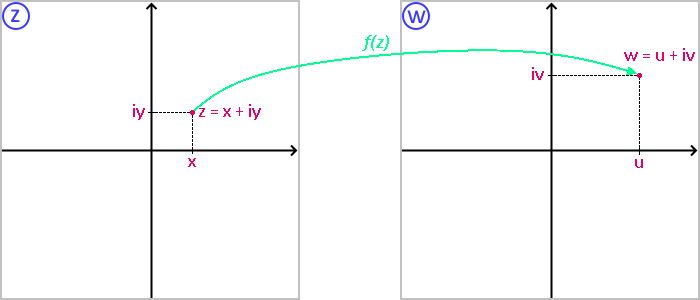
\includegraphics[height=0.4\textwidth]{lec25_2.png}
 
 Соответствующие свойства сходимости и непрерывности общих ФКП \eqref{lec25:3}
 определяются через аналогичные свойства действительных Ф2П.
 Свойства дифференцируемости и интегрируемости ФКП \eqref{lec25:3} несколько
 отличаются от соответствующих свойств действительных Ф2П и будут
 рассмотрены позже.
 
 К \emph{простейшим ФКП} будем относить \emph{линейниые},  
 \emph{дробные},  \emph{степенные},  \emph{тригонометрические} и 
 \emph{гиперболические},
 а также обратные к ним, \emph{экспоненциальные},
 \emph{общепоказательные} и \emph{логарифмические ФКП}.

 \subsection{Линейная ФКП}
\begin{equation}
\label{lec25:4}
\begin{cases} 
  w = az + b\\
  \fix{a, b} \in \C
\end{cases}
\end{equation}
	\begin{enumerate}
	\item Если $a = 0$, то $w \overset{\eqref{lec25:4}}{=} b = const$
	
	 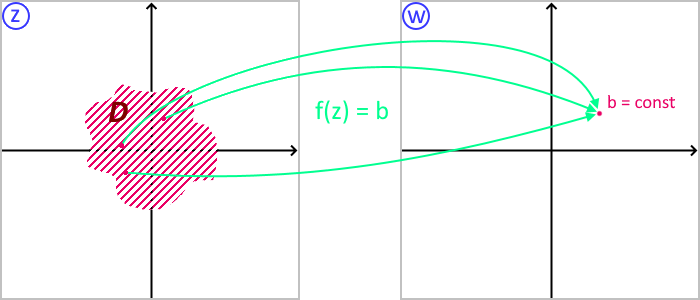
\includegraphics[width=0.9\textwidth]{lec25_3.png}
	
\item Если $a \ne 0$, то $\eqref{lec25:4} \implies z = \frac{w - b}{a}=
\alpha{w} + \beta,\ \text{где}\
	\begin{cases} 
 	 \alpha = \frac{1}{a} \ne 0\\
  	\beta =  -\frac{b}{a} \in \C
	\end{cases}$
		\begin{enumerate}
			\item Если $b = 0$, то \begin{equation}
			\label{lec25:5}
			w = az
			\end{equation}
			$
			\begin{cases} 
 	 		|w|= |a| \cdot |z| = k \cdot |z|\\
  			k =|a| > 0
			\end{cases}
			$\hspace{-1em} --- это соответствует растяжению/сжатию в $k$ раз 
			линии из \textcircled{z} в \textcircled{w}
			(аналогично для 
			более сложных фигур).
			
			
			Параметрически, мы получаем преобразование подобия с возможным поворотом на
соответствующий угол. Для этого использовав экспоненциальную форму, имеем:
			\[\begin{gathered}
			\begin{cases} 
 	 		a = |a| \cdot e^{i\phi_0}, \ \phi_0 = \arg{a} \\
 	 		z = re^{i\phi}\\
 	 		r = |z|,\  \phi = \Arg z
			\end{cases}\implies
			w = |a| \cdot re^{i(\phi + \phi_0)}\implies\\\implies
			\begin{cases} 
 	 		|w|= k|z| \\
 	 		\Arg w = \phi + \phi_0 \text{ --- поворот на }\phi_0\\
 	 		k = |a| > 0 \text{ --- коэффициент подобия}
			\end{cases}
			\end{gathered}\]
			
			 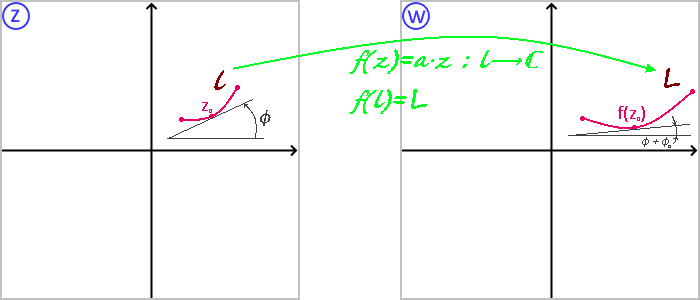
\includegraphics[width=0.9\textwidth]{lec25_4.png}
			 
			 \item Если $a = 1$, то получаем $w = z + b$. В таком случае имеем 
			 параллельный перенос на вектор, соответствующий
радиус-вектору числа $b$.
			
			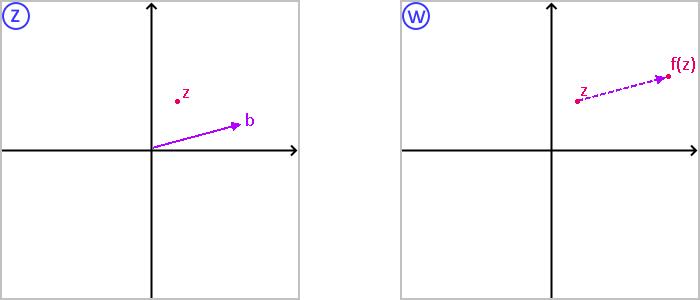
\includegraphics[width=0.9\textwidth]{lec25_5.png}
		\end{enumerate}
В общем случае для $a \ne 0$ общую линейную ФКП можно записать в следующем 
виде:
		\[
	           w = az + b = a\left(z + \frac{b}{a}\right) = a(z + z_0).
		\]
Применим линейную ФКП сначала к вектору $w_1 = z + z_0$ --- параллельному
переносу $z$ на радиус-вектор числа $z_0 = \frac{b}{a}$.
		 Получим $w = aw_1$, где:
		 \[
		 a = |a|e^{i\phi_0},\ k = |a| > 0 \implies 
		 \begin{cases}
		 w = kw_2 \text{ --- подобие} \\
		 w_2 = e^{i\phi_0}w_1  \text{ --- поворот}
		 \end{cases}
		 \]
		
Образ любой линейной ФКП получается с помощью линейного переноса,
растяжения/сжатия и поворота.
		\end{enumerate}
\subsection{Дробно-линейная ФКП}
	\begin{equation}
	\label{lec25:7}
	w = \frac{az + b}{cz + d},\  \text{где} \fix{a, b, c, d} \in \C,
	\end{equation}
	причем либо $c \ne 0$, либо $d \ne 0$.
	
Если $c = 0,\ d \ne 0$, то $w \overset{\eqref{lec25:7}}{=} \dfrac{az + b}{d} =
a_0{z} + b_0, \
	\begin{cases} 
 	 a_0  = \frac{a}{d} \in \C\\
  	 b_0  = \frac{b}{d} \in \C
	\end{cases}\hspace{-1em}
$ --- переходим к линейной ФКП. 

Если в \eqref{lec25:7} $\Delta = \begin{vmatrix}a&b\\
c&d\end{vmatrix} = ad - bc = 0$, то \eqref{lec25:7} сводится к константной 
ФКП~--- частный случай линейной ФКП.
	 
	Пусть  $\Delta \ne 0,\ c \ne 0$. Тогда имеем:
	\begin{equation}
	\label{lec25:8}
w \overset{\eqref{lec25:7}}{=} \frac{a}{c} - \frac{\Delta}{c^{2}(z +
\frac{d}{c})}
	\end{equation}
	
\eqref{lec25:8} можно представить как последовательное применение следующих
отображений:
		 \begin{enumerate}
	 	\item 
	 	$ \begin{cases} 
 	 	w_1 = z + z_0\\
  	  	z_0 = \frac{d}{c} \in \C
		\end{cases}$ --- паралелльный перенос на радиус-вектор числа $z_0$,
\item $w_2 = \frac{1}{w_1}$ --- инверсия (подобие относительно единичной
окружности),
		\item 
		$ \begin{cases} 
 	 	w_3 = pw_2\\
  	  	p = -\frac{\Delta}{c^2} \ne 0
		\end{cases}$ --- растяжение/сжатие и поворот,
		\item 
		$ \begin{cases} 
 	 	w_4 = w_3 + w_0\\
  	  	w_0 = \frac{a}{c} \ne 0
		\end{cases}$ --- параллельный перенос.
	 	 \end{enumerate}
 
 Из указанного отображения новой является лишь операция инверсии относительно
 единичной окружности.
\end{document}
